\documentclass[11pt,a4paper]{article}

% ---------- Język i kodowanie ----------
\usepackage{iftex}
\ifPDFTeX                      % pdfLaTeX (m.in. domyslny silnik Overleafa)
  \usepackage[T1]{fontenc}
  \usepackage[utf8]{inputenc}
  \usepackage{lmodern}
  \newcommand{\tptimes}{\fontfamily{qtm}\selectfont}   % TeX Gyre Termes (Times)
\else                          % XeLaTeX / LuaLaTeX / Tectonic
  \usepackage{fontspec}
  \setmainfont{lmroman10-regular.otf}[
    BoldFont=lmroman10-bold.otf, ItalicFont=lmroman10-italic.otf,
    BoldItalicFont=lmroman10-bolditalic.otf]
  \setmonofont{lmmono10-regular.otf}
  \newfontfamily\tptimes{texgyretermes-regular.otf}[
    BoldFont=texgyretermes-bold.otf, ItalicFont=texgyretermes-italic.otf,
    BoldItalicFont=texgyretermes-bolditalic.otf]
\fi
\usepackage[polish]{babel}

% ---------- Matematyka, grafika, tabele ----------
\usepackage{amsmath}
\usepackage{amssymb}
\usepackage{graphicx}
\usepackage{booktabs}
\usepackage{float}
\usepackage{longtable}
\makeatletter
\setlength{\@fptop}{0pt}
\setlength{\@fpsep}{14pt plus 1fil}
\setlength{\@fpbot}{0pt plus 1fil}
\makeatother
\usepackage{caption}
\captionsetup[table]{position=top}
\captionsetup[figure]{position=bottom}
\usepackage{multirow}
\usepackage{array}
\usepackage{colortbl}
\usepackage[margin=2.5cm]{geometry}
\usepackage{pgfplots}
\pgfplotsset{compat=1.18}

% Barwy serii (rozróżnialne także w druku cz.-b. dzięki stylom linii)
\definecolor{seriaA}{HTML}{1F5FA9}   % niebieski
\definecolor{seriaB}{HTML}{C62828}   % czerwony
\definecolor{seriaC}{HTML}{2E7D32}   % zielony
\definecolor{seriaD}{HTML}{E07B00}   % pomarańczowy
\definecolor{seriaE}{HTML}{6A3D9A}   % fioletowy
\definecolor{dynam}{HTML}{555555}    % szary -- zakres dynamiki
\pgfplotsset{
  wykres/.style={
    width=15.2cm, height=8.4cm, grid=major,
    grid style={line width=0.2pt, draw=gray!18},
    major grid style={line width=0.35pt, draw=gray!30},
    xlabel={Częstotliwość $f$ [GHz]}, xmin=0.8, xmax=5.8,
    xtick={1,1.5,2,2.5,3,3.5,4,4.5,5,5.5},
    x tick label style={/pgf/number format/use comma},
    y tick label style={/pgf/number format/use comma},
    legend cell align=left,
    legend style={font=\small, fill=white, draw=gray!40, at={(0.5,0)}, anchor=north, yshift=-1.25cm,
                  /tikz/every even column/.append style={column sep=1.0em}},
    title style={font=\small, yshift=0.2em},
    tick label style={font=\small}, label style={font=\small}
  }
}
\usepackage[hidelinks,unicode]{hyperref}
\emergencystretch=1em
% Wstawianie wierszy tabel z plików: prymityw TeX-a działa w tabular przed \bottomrule
\makeatletter\newcommand{\tabinput}[1]{\@@input #1.tex }\makeatother

% ---------- Strona tytułowa: odwzorowanie Szablon_strony_tytulowej_LKEMBEM.doc ----------
\newcolumntype{Y}[1]{>{\centering\arraybackslash}m{#1}}
\newcolumntype{Z}[1]{>{\raggedright\arraybackslash}m{#1}}
\newcolumntype{W}[1]{>{\raggedright\arraybackslash}p{#1}}
\newlength{\tpw}\newlength{\tpt}
\newlength{\tpcA}\newlength{\tpcB}\newlength{\tpcC}
\newlength{\tpAB}\newlength{\tpBC}\newlength{\tpABC}
\newlength{\tpsig}
\newcommand{\tplengths}{%
  \setlength{\tabcolsep}{5pt}%
  \setlength{\arrayrulewidth}{0.5pt}%
  \setlength{\tpw}{\dimexpr\textwidth-4\arrayrulewidth-6\tabcolsep-1pt\relax}%
  \setlength{\tpcA}{0.4966\tpw}%
  \setlength{\tpcB}{0.2481\tpw}%
  \setlength{\tpcC}{0.2553\tpw}%
  \setlength{\tpAB}{\dimexpr\tpcA+\tpcB+2\tabcolsep+\arrayrulewidth\relax}%
  \setlength{\tpBC}{\dimexpr\tpcB+\tpcC+2\tabcolsep+\arrayrulewidth\relax}%
  \setlength{\tpABC}{\dimexpr\tpAB+\tpcC+2\tabcolsep+\arrayrulewidth\relax}%
  \setlength{\tpsig}{\dimexpr(\tpABC-2\arrayrulewidth)/3\relax}}
\newcommand{\tph}[1]{\setlength{\tpt}{#1}\rule[-0.5\tpt]{0pt}{\tpt}}

% ---------- Dane do strony tytułowej ----------
\newcommand{\tpTermin}{PN/N, 15.15 - 18.45}
\newcommand{\tpGrupa}{5}
\newcommand{\tpCwiczenie}{1}
\newcommand{\tpTemat}{Badanie skuteczności ekranowania barier (przesłony, szczeliny)}
\newcommand{\tpDataWyk}{26.10.2026}
\newcommand{\tpDataOdd}{08.11.2026}             % SPRAWDZIĆ przed oddaniem
\newcommand{\tpWersja}{Oryginał}
\newcommand{\tpAutor}{Wiktor Gruszczyński, 283808}
\newcommand{\tpWspolautorA}{Nikodem Konieczny, 283838}
\newcommand{\tpWspolautorB}{Filip Rodziewicz, 283825}
\newcommand{\tpAutorPodpis}{Wiktor Gruszczyński}
\newcommand{\tpWspolautorAPodpis}{Nikodem Konieczny}
\newcommand{\tpWspolautorBPodpis}{Filip Rodziewicz}

\newcommand{\stronatytulowa}{%
\begin{titlepage}
\thispagestyle{empty}
\tptimes\fontsize{12}{14.4}\selectfont
\tplengths
\arrayrulecolor[HTML]{BFBFBF}
\noindent
\begin{tabular}{|Z{\tpcA}|Z{\tpcB}|Z{\tpcC}|}
\hline
\multicolumn{3}{|Y{\tpABC}|}{%
  \textbf{\textsc{Politechnika Wrocławska}}\newline
  \textbf{\textsc{Katedra Telekomunikacji i~Teleinformatyki}}} \\
\hline
\multicolumn{1}{|Y{\tpcA}|}{\vspace*{3pt}%
  \textbf{\textsc{Bezpieczeństwo elektromagnetyczne}}\vspace*{3pt}} &
\multicolumn{2}{Y{\tpBC}|}{\textsc{Termin zajęć: \tpTermin}} \\
\hline
\tph{20pt}\textsc{Nr grupy:} \textbf{\tpGrupa} &
\multicolumn{2}{Z{\tpBC}|}{\textsc{Nr ćwiczenia:} \textbf{\tpCwiczenie}} \\
\hline
\multicolumn{1}{|W{\tpcA}|}{%
  \textsc{Skład grupy:}\newline
  \underline{\textsc{\tpAutor}}\newline
  \textsc{\tpWspolautorA}\newline
  \textsc{\tpWspolautorB}\vspace*{6pt}} &
\multicolumn{2}{W{\tpBC}|}{\multirow[t]{3}{\tpBC}{%
  \textsc{Temat ćwiczenia:}\newline
  \textbf{\textsc{\tpTemat}}}} \\
\cline{1-1}
\multicolumn{1}{|Z{\tpcA}|}{\tph{22pt}%
  \textsc{Data wykonania ćw.:} \textbf{\tpDataWyk}} &
\multicolumn{2}{Z{\tpBC}|}{} \\
\cline{1-1}
\multicolumn{1}{|Z{\tpcA}|}{\vspace*{3pt}%
  \textsc{Wersja sprawozdania:}\newline
  \hfill\textbf{\textsc{\tpWersja}}\vspace*{3pt}} &
\multicolumn{2}{Z{\tpBC}|}{} \\
\hline
\multicolumn{2}{|Z{\tpAB}|}{\tph{26pt}\textsc{Data oddania sprawozdania:} \textbf{\tpDataOdd}} &
  \textsc{Ocena:} \\
\hline
\multicolumn{3}{|Y{\tpABC}|}{\tph{26pt}%
  \textbf{Zapoznałem się z~niniejszym sprawozdaniem i~uważam je za wykonane poprawnie.}} \\
\hline
\multicolumn{3}{|Y{\tpABC}|}{\setlength{\tabcolsep}{0pt}%
  \begin{tabular}{@{}Y{\tpsig}|Y{\tpsig}|Y{\tpsig}@{}}
    \tph{28pt}\fontsize{10}{12}\selectfont\tpAutorPodpis &
    \fontsize{10}{12}\selectfont\tpWspolautorAPodpis &
    \fontsize{10}{12}\selectfont\tpWspolautorBPodpis
  \end{tabular}} \\
\hline
\end{tabular}
\arrayrulecolor{black}
\end{titlepage}}

% Wspólny nagłówek tabel z wynikami w funkcji częstotliwości
\newcommand{\naglPrzeslony}{%
  $f$ & 100$\times$1 & 16$\times$2 & 16$\times$3 & 100$\times$3 & 4$\times$6 & 36$\times$6
      & 16$\times$8 & 1$\times$12 & 4$\times$12}

\addto\captionspolish{\renewcommand{\refname}{Bibliografia}}
\begin{document}
\stronatytulowa

\section{Cel ćwiczenia}

Cel ćwiczenia sformułowano w~instrukcji~\cite[rozdz.~1]{instr} następująco:
\begin{quote}
\emph{„Celem ćwiczenia jest praktyczne zapoznanie się z~techniką pomiaru skuteczności
ekranowania przesłon i~szczelin. W~ramach ćwiczenia doskonalone będą umiejętności
posługiwania się aparaturą pomiarową oraz zestawiania toru pomiarowego. Ćwiczenie ma na
celu zapoznanie się z~metodą pomiaru oraz pokazanie jak istotny jest wpływ właściwego
zamontowanie badanych przesłon oraz układów do pomiaru referencyjnego na dokładność
uzyskiwanych wyników.”}~\cite{instr}
\end{quote}
Badaniu poddano dziewięć przesłon z~otworami okrągłymi oraz dwie szczeliny o~szerokości
$1{,}5\ \mathrm{cm}$ i~$1{,}8\ \mathrm{cm}$.

\section{Stanowisko pomiarowe}

\subsection{Metoda pomiarowa}

Zastosowano metodę porównawczą opisaną w~normie IEEE Std~299~\cite{ieee299}. Antena nadawcza
znajduje się na zewnątrz komory ekranowanej, a~antena odbiorcza wewnątrz, naprzeciw okna
pomiarowego~\cite[p.~2.2]{instr}. Wektorowy analizator sieci mierzy współczynnik transmisji
między antenami. Antena odbiorcza była podłączona do portu~1, a~nadawcza do portu~2, dlatego
mierzono parametr $S_{12}$, czyli stosunek fali odebranej na porcie~1 do fali pobudzającej
port~2~\cite[p.~3.1]{instr}. Skuteczność ekranowania wyznacza się z~różnicy poziomów
zmierzonych bez przesłony i~z~przesłoną, przy niezmienionym położeniu anten.

\subsection{Konfiguracja stanowiska pomiarowego}

\subsubsection{Spis aparatury pomiarowej}

\begin{table}[H]
  \centering
  \small
  \caption{Spis aparatury i~wyposażenia stanowiska pomiarowego.}
  \label{tab:aparatura}
  \renewcommand{\arraystretch}{1.25}
  \begin{tabular}{|c|>{\raggedright\arraybackslash}p{4.6cm}|>{\raggedright\arraybackslash}p{8.2cm}|}
    \hline
    \textbf{Lp.} & \textbf{Nazwa przyrządu / elementu} & \multicolumn{1}{c|}{\textbf{Model lub typ, uwagi}} \\
    \hline
    1 & Wektorowy analizator sieci (VNA)
      & Tektronix TTR506A, 100~kHz--6~GHz, obsługa z~komputera
        w~programie VectorVu-PC~\cite{ttr500} \\
    \hline
    2 & Antena nadawcza & antena logarytmiczno-periodyczna na statywie,
        na zewnątrz komory, port~2 \\
    \hline
    3 & Antena odbiorcza & antena logarytmiczno-periodyczna na płytce drukowanej,
        wewnątrz komory, port~1 \\
    \hline
    4 & Komora ekranowana & okrągłe okno pomiarowe w~ścianie, nieszczelności
        wypełnione wełną stalową \\
    \hline
    5 & Przewody antenowe & współosiowe, ekranowane \\
    \hline
    6 & Pełna przesłona metalowa & do pomiaru zakresu dynamiki \\
    \hline
    7 & Badane przesłony & 9 blach z~otworami okrągłymi, tab.~\ref{tab:probki} \\
    \hline
    8 & Blachy do formowania szczelin & 2 arkusze nasuwane symetrycznie na okno \\
    \hline
    9 & Rama dociskowa ze sklejki i~ściski & docisk przesłony do ściany komory \\
    \hline
  \end{tabular}
\end{table}

Niepewność wnoszona przez sam analizator jest pomijalna, ponieważ szum śladu TTR506A
wynosi typowo $0{,}006\ \mathrm{dB}$~RMS w~paśmie od $200\ \mathrm{MHz}$ do
$6\ \mathrm{GHz}$~\cite{ttr500}. O~niepewności wyniku decydują odbicia fal w~pomieszczeniu
oraz powtarzalność montażu przesłony. Ich wpływ omówiono w~rozdziale~\ref{sec:analiza}.

\subsubsection{Opis konfiguracji}

Analizator ustawiono przy komorze, aby przewody antenowe były jak najkrótsze. Antena
odbiorcza stała na podstawie wewnątrz komory, a~antena nadawcza na statywie na zewnątrz.
Obie anteny skierowano na środek okna pomiarowego. Badane przesłony dociskano do ściany
komory ramą ze sklejki i~ściskami, aby zapewnić kontakt galwaniczny na całym obwodzie okna.
Zakres częstotliwości dobrano na podstawie charakterystyk dopasowania anten
(rys.~\ref{fig:dopasowanie}). Antenę uznaje się za dopasowaną, gdy jej współczynnik odbicia
nie przekracza $-10\ \mathrm{dB}$~\cite[rozdz.~5]{instr}.

\begin{figure}[htbp]
  \centering
  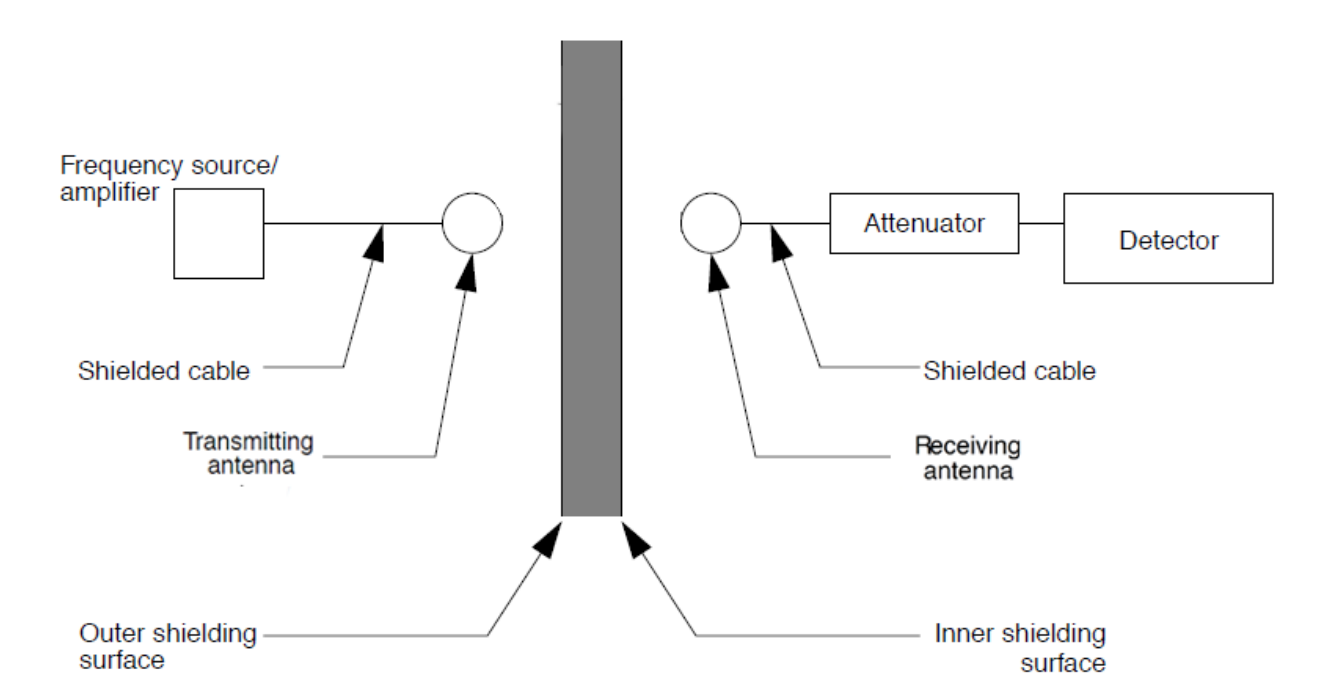
\includegraphics[width=0.78\textwidth]{rys/schemat_stanowiska.png}
  \caption{Ogólny schemat stanowiska do wyznaczania skuteczności ekranowania
           wg~\cite[rys.~2-3]{instr}, za~\cite{ieee299}.}
  \label{fig:schemat}
\end{figure}

\begin{figure}[htbp]
  \centering
  \begin{minipage}[t]{0.56\textwidth}\centering
    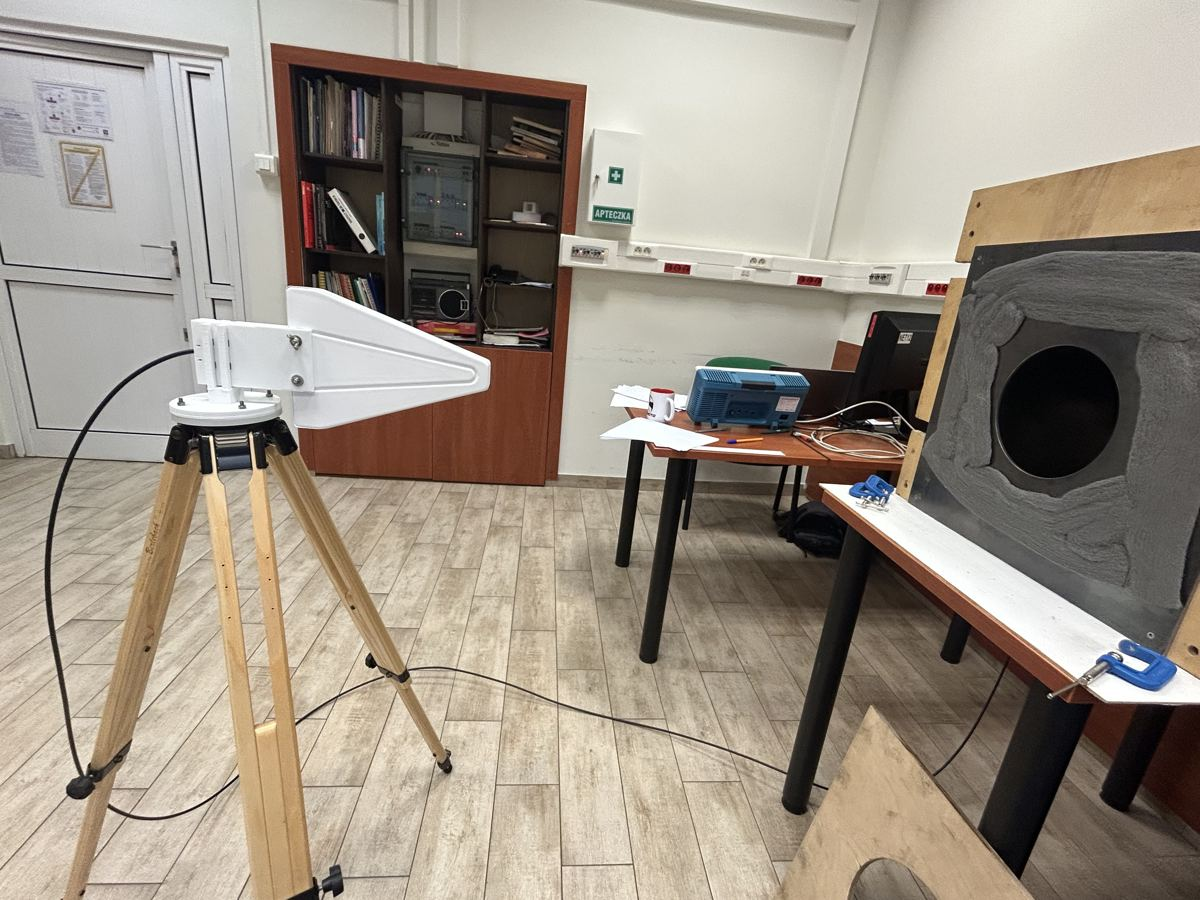
\includegraphics[width=\linewidth]{rys/stanowisko.jpg}\\[-1pt]
    {\small a) antena nadawcza i~komora z~oknem pomiarowym}
  \end{minipage}\hfill
  \begin{minipage}[t]{0.41\textwidth}\centering
    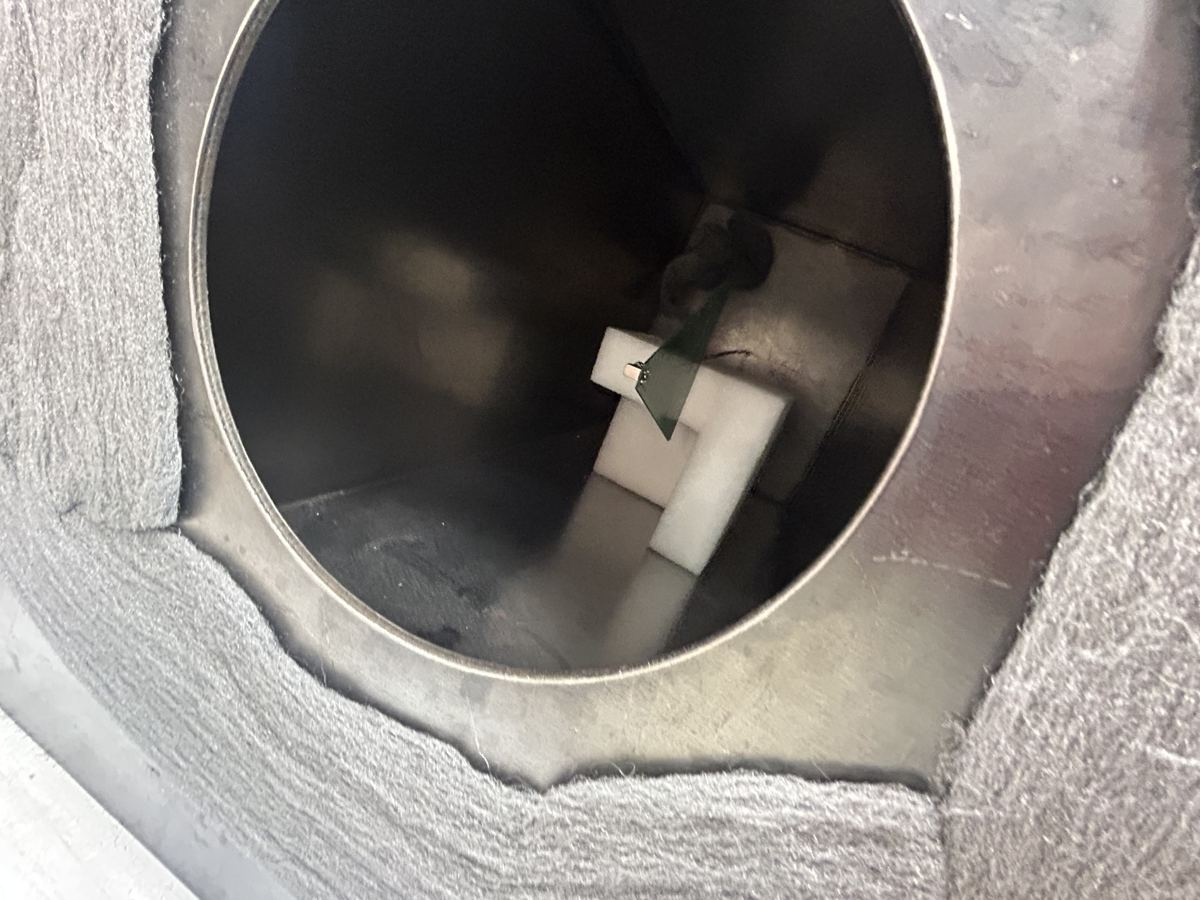
\includegraphics[width=\linewidth]{rys/antena_odbiorcza.jpg}\\[-1pt]
    {\small b) antena odbiorcza wewnątrz komory}
  \end{minipage}
  \caption{Stanowisko pomiarowe w~sali~347 bud.~C-4, zdjęcia własne z~26.10.2026.}
  \label{fig:stanowisko}
\end{figure}

\begin{figure}[htbp]
  \centering
  \begin{minipage}[t]{0.49\textwidth}\centering
    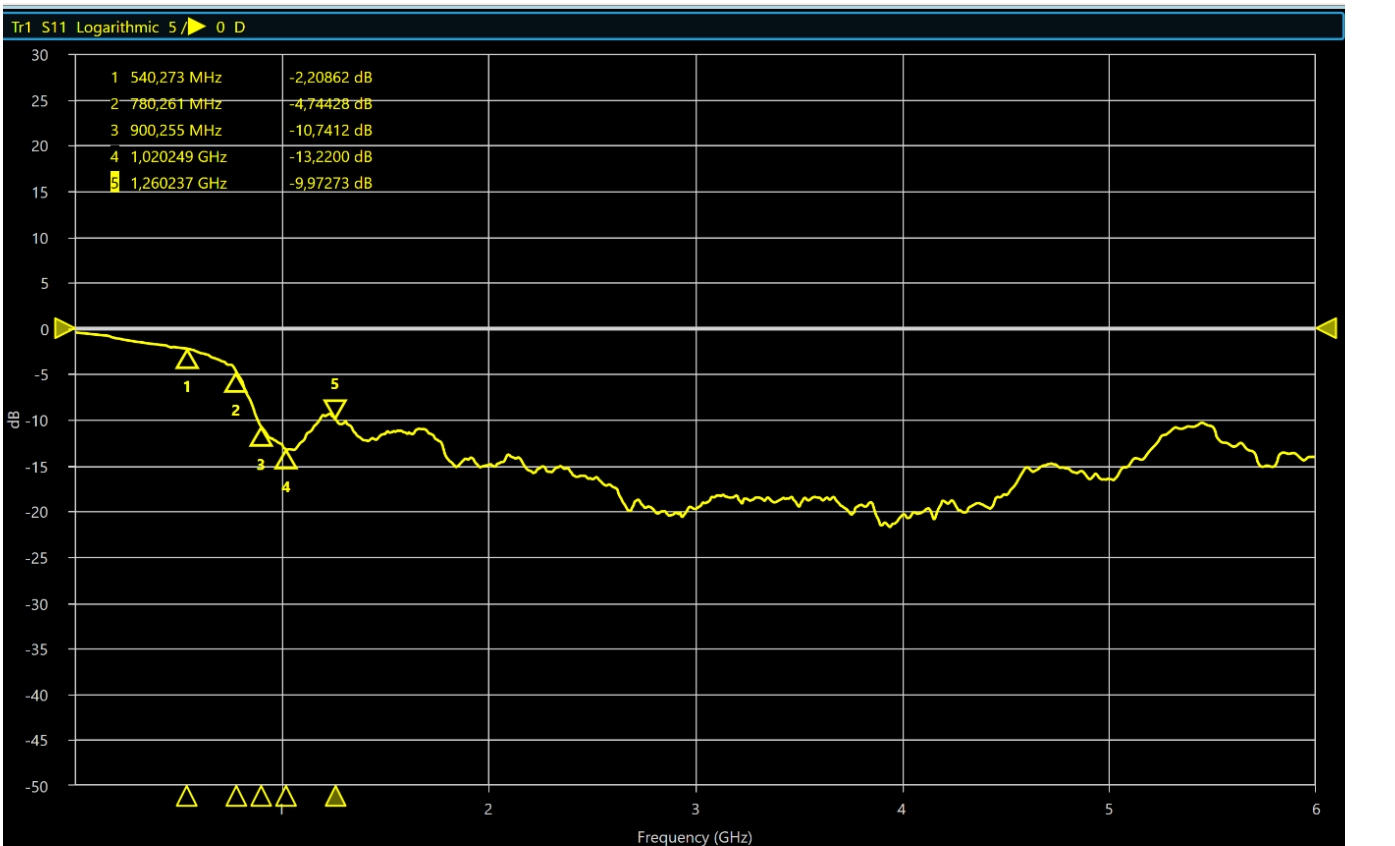
\includegraphics[width=\linewidth]{rys/dopasowanie_wewn.png}\\
    {\small a) antena wewnątrz komory, $S_{11}$}
  \end{minipage}\hfill
  \begin{minipage}[t]{0.49\textwidth}\centering
    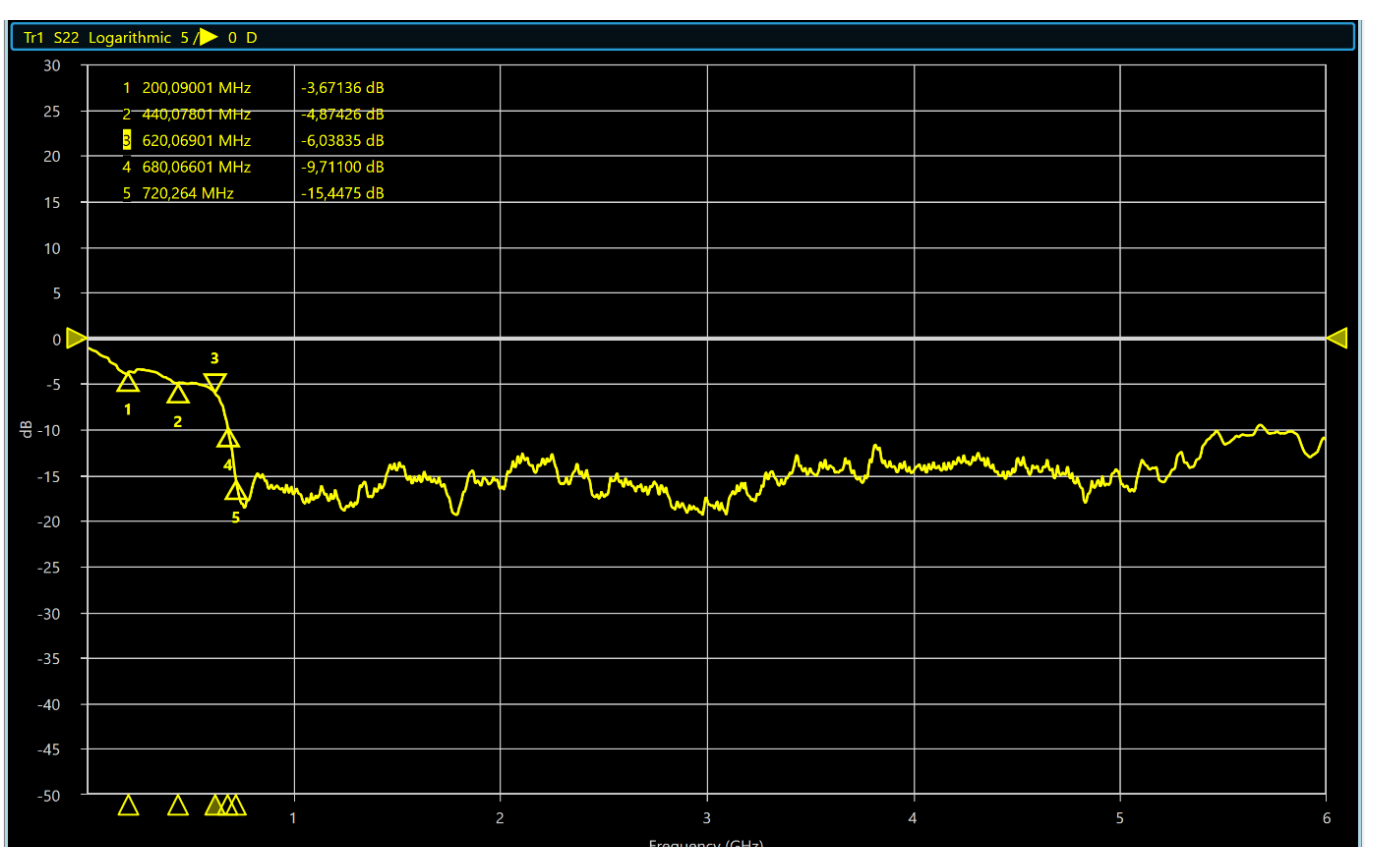
\includegraphics[width=\linewidth]{rys/dopasowanie_zewn.png}\\
    {\small b) antena zewnętrzna, $S_{22}$}
  \end{minipage}
  \caption{Charakterystyki dopasowania anten stanowiska wg~\cite[rys.~5-2 i~5-3]{instr}.
           Antena zewnętrzna jest dopasowana od ok.~$0{,}7\ \mathrm{GHz}$, a~antena wewnętrzna
           w~paśmie $0{,}9$--$1{,}0\ \mathrm{GHz}$ oraz od $1{,}26$ do ok.~$5{,}3\ \mathrm{GHz}$.}
  \label{fig:dopasowanie}
\end{figure}

\section{Realizacja ćwiczenia}

\subsection{Nastawy analizatora i~źródło danych}

\paragraph{Uwaga metodyczna.} Podczas zajęć wyniki zapisano poleceniem \emph{Save State}
zamiast \emph{Save SnP}. Pliki \texttt{.cstate} w~protokole zawierają przez to tylko
nastawy i~kalibrację przyrządu, bez przebiegów $S_{12}$. Na polecenie prowadzącego
sprawozdanie opracowano na danych przekazanych przez prowadzącego~\cite{dane}. Pomiar
wykonano na tym samym stanowisku i~dla tego samego zestawu przesłon, przy odległości anten
$1{,}8\ \mathrm{m}$ i~polaryzacji pionowej. Opis stanowiska, nastawy przyrządu, zdjęcia
i~wymiary próbek pochodzą z~zajęć grupy~5. Nastawy z~obu źródeł zestawiono
w~tabeli~\ref{tab:nastawy}.

\begin{table}[H]
  \centering
  \small
  \caption{Nastawy wektorowego analizatora sieci.}
  \label{tab:nastawy}
  \renewcommand{\arraystretch}{1.15}
  \begin{tabular}{|l|>{\centering\arraybackslash}p{5.3cm}|>{\centering\arraybackslash}p{4.6cm}|}
    \hline
    \textbf{Parametr} & \textbf{Zajęcia gr.~5 (pliki \texttt{.cstate})} & \textbf{Dane opracowane~\cite{dane}} \\
    \hline
    Mierzony parametr      & $S_{12}$ & $S_{12}$ oraz $S_{22}$ \\
    \hline
    Zakres częstotliwości  & $1{,}26$--$5{,}30\ \mathrm{GHz}$ & $0{,}80$--$5{,}80\ \mathrm{GHz}$ \\
    \hline
    Liczba punktów / krok  & 201 / $20{,}2\ \mathrm{MHz}$ & 201 / $25\ \mathrm{MHz}$ \\
    \hline
    Szerokość pasma IF     & $10\ \mathrm{kHz}$ & nie podano, przyjęto $10\ \mathrm{kHz}$ \\
    \hline
    Moc wyjściowa portu    & $0\ \mathrm{dBm}$ & nie podano, przyjęto $0\ \mathrm{dBm}$ \\
    \hline
    Uśrednianie            & współczynnik~5~\cite[p.~3.1.1]{instr} & nie podano \\
    \hline
    Odległość anten / polaryzacja & nie zapisano & $1{,}8\ \mathrm{m}$ / pionowa \\
    \hline
    Format zapisu          & stan przyrządu \texttt{.cstate} & Touchstone \texttt{.s2p}, RI \\
    \hline
  \end{tabular}
\end{table}

\subsection{Badane próbki}

Przesłony oznaczono tak jak w~danych~\cite{dane} symbolem $N\times d$, gdzie $N$ to liczba
otworów, a~$d$ nominalna średnica otworu w~centymetrach. W~tabeli~\ref{tab:probki} podano
również średnice zmierzone przez grupę wraz z~numerami płyt z~zajęć oraz częstotliwość
graniczną $f_g$ ze wzoru~\eqref{eq:fg}, powyżej której otwór przestaje tłumić falę.

\begin{table}[H]
  \centering
  \small
  \caption{Badane próbki: liczba otworów, średnica nominalna i~zmierzona, częstotliwość graniczna.}
  \label{tab:probki}
  \renewcommand{\arraystretch}{1.15}
  \begin{tabular}{|c|c|c|c|c|c|}
    \hline
    \textbf{Oznaczenie} & \textbf{Nr płyty} & $N$ & $d_{nom}$ [cm] & $d_{zm}$ [cm] & $f_g$ [GHz] \\
    \hline
    100$\times$1 & 6 & 100 & 1   & 1,4  & 14,99 \\ \hline
    16$\times$2  & 1 & 16  & 2   & 2,0  & 7,49 \\ \hline
    16$\times$3  & 8 & 16  & 3   & 3,2  & 5,00 \\ \hline
    100$\times$3 & 3 & 100 & 3   & 3,5  & 5,00 \\ \hline
    4$\times$6   & 7 & 4   & 6   & 7,0  & 2,50 \\ \hline
    36$\times$6  & 2 & 36  & 6   & 6,0  & 2,50 \\ \hline
    16$\times$8  & 5 & 16  & 8   & 8,3  & 1,87 \\ \hline
    1$\times$12  & 4 & 1   & 12  & 12,5 & 1,25 \\ \hline
    4$\times$12  & 9 & 4   & 12  & 17,0 & 1,25 \\ \hline
    Szczelina    & --- & --- & \multicolumn{2}{c|}{szer. 1,5 oraz 1,8} & --- \\ \hline
  \end{tabular}
\end{table}

Numery płyt przyporządkowano oznaczeniom na podstawie zdjęć, porównując liczbę i~rozmiar
otworów. Średnice mierzono linijką przez okno w~ramie dociskowej, która częściowo zasłaniała
otwory. Stąd biorą się różnice względem wartości nominalnych, największe dla płyty~9
o~nachodzących na siebie otworach i~dla płyty~4, zmierzonej niecentrycznie. W~obliczeniach
przyjęto wartości nominalne.

\begin{figure}[htbp]
  \centering
  \newcommand{\fot}[2]{\begin{minipage}[t]{0.19\textwidth}\centering
      \includegraphics[height=3.6cm,width=\linewidth,keepaspectratio]{rys/#1.jpg}\\{\footnotesize #2}\end{minipage}}
  \fot{przeslona_100x1}{a) 100$\times$1}\hfill
  \fot{przeslona_16x2}{b) 16$\times$2}\hfill
  \fot{przeslona_16x3}{c) 16$\times$3}\hfill
  \fot{przeslona_100x3}{d) 100$\times$3}\hfill
  \fot{przeslona_4x6}{e) 4$\times$6}\\[6pt]
  \fot{przeslona_36x6}{f) 36$\times$6}\hfill
  \fot{przeslona_16x8}{g) 16$\times$8}\hfill
  \fot{przeslona_4x12}{h) 4$\times$12}\hfill
  \fot{szczelina_pionowa}{i) szczelina pionowa}\hfill
  \fot{szczelina_pozioma}{j) szczelina pozioma}
  \caption{Zamontowane próbki, zdjęcia własne z~26.10.2026. Przesłony sfotografowano w~ramie
           dociskowej lub przed montażem. Dla przesłony 1$\times$12 zdjęcia nie wykonano.}
  \label{fig:probki}
\end{figure}

\subsection{Pomiar referencyjny i~pomiar zakresu dynamiki}

Pomiar referencyjny wykonano przy otwartym oknie komory, bez przesłony. Następnie, przy tym
samym położeniu anten, okno zamknięto pełną przesłoną metalową i~zmierzono zakres dynamiki
stanowiska, czyli najmniejszy poziom sygnału, jaki dociera do anteny odbiorczej przy
szczelnie zamkniętym oknie~\cite[p.~2.2.3]{instr}.

\subsection{Pomiary przesłon i~szczelin}

Każdą przesłonę montowano centrycznie w~oknie i~dociskano do ściany komory~\cite[p.~3.4]{instr}.
Szczeliny tworzono, nasuwając symetrycznie dwie blachy z~obu stron okna tak, aby szczelina
o~zadanej szerokości powstała w~jego środku~\cite[p.~3.5]{instr}. Położenie anten nie
zmieniało się w~trakcie wszystkich pomiarów.

\subsection{Wyniki pomiarów}

Analizator zapisuje parametr $S_{12}$ jako liczbę zespoloną. Jego moduł w~decybelach
obliczono ze wzoru:
\begin{equation}
  |S_{12}|\,[\mathrm{dB}] = 20\log_{10}\sqrt{(\operatorname{Re} S_{12})^2 + (\operatorname{Im} S_{12})^2}.
  \label{eq:s12db}
\end{equation}
Tabele~\ref{tab:s12ref} i~\ref{tab:s12przeslony} zawierają wartości dla wybranych
częstotliwości. Pełne przebiegi, po 201 punktów, przedstawiono na wykresach
w~rozdziale~\ref{sec:analiza}.

\begin{table}[H]
  \centering
  \small
  \caption{Wyniki pomiarów $S_{12}$: pomiar referencyjny (część rzeczywista, urojona i~moduł),
           pomiar dynamiki oraz pomiary szczelin.}
  \label{tab:s12ref}
  \renewcommand{\arraystretch}{1.1}
  \begin{tabular}{rrrrrrr}
    \toprule
    $f$ & $\operatorname{Re} S_{12,\mathrm{ref}}$ & $\operatorname{Im} S_{12,\mathrm{ref}}$
        & $S_{12,\mathrm{ref}}$ & $S_{12,\mathrm{dyn}}$ & $S_{12,\mathrm{sz}1,5}$ & $S_{12,\mathrm{sz}1,8}$ \\
    $[\mathrm{GHz}]$ & [--] & [--] & [dB] & [dB] & [dB] & [dB] \\
    \midrule
    \tabinput{tabele/t_s12_ref}
    \bottomrule
  \end{tabular}
\end{table}

\paragraph{Przykład obliczeń do tabeli~\ref{tab:s12ref}.} Dla pomiaru referencyjnego przy
$f = 0{,}80\ \mathrm{GHz}$:
\[
  |S_{12,\mathrm{ref}}| = 20\log_{10}\sqrt{(-0{,}02060)^2 + (-0{,}01059)^2}
  = 20\log_{10}(0{,}02316) = -32{,}70\ \mathrm{dB} \approx -32{,}7\ \mathrm{dB}.
\]
Pozostałe kolumny obliczono tak samo. W~tabeli podano wartości zaokrąglone do $0{,}1\ \mathrm{dB}$.

\begin{table}[H]
  \centering
  \small
  \caption{Wyniki pomiarów $S_{12}$ [dB] dla przesłon $N\times d$, częstotliwość $f$ w~GHz.}
  \label{tab:s12przeslony}
  \renewcommand{\arraystretch}{1.1}
  \begin{tabular}{rrrrrrrrrr}
    \toprule
    \naglPrzeslony \\
    \midrule
    \tabinput{tabele/t_s12_przeslony}
    \bottomrule
  \end{tabular}
\end{table}

\paragraph{Przykład obliczeń do tabeli~\ref{tab:s12przeslony}.} Dla przesłony 100$\times$1
przy $f = 1{,}00\ \mathrm{GHz}$, gdzie $\operatorname{Re} S_{12} = 3{,}735\cdot10^{-4}$
i~$\operatorname{Im} S_{12} = -0{,}608\cdot10^{-4}$:
\begin{align*}
  |S_{12}| &= 20\log_{10}\sqrt{(3{,}735\cdot10^{-4})^2+(-0{,}608\cdot10^{-4})^2}\\
  &= 20\log_{10}(3{,}784\cdot10^{-4}) = -68{,}44\ \mathrm{dB} \approx -68{,}4\ \mathrm{dB}.
\end{align*}

\subsection{Wyznaczenie skuteczności ekranowania}

Skuteczność ekranowania dla pola elektrycznego zdefiniowana jest zależnością~\cite[wzór~(1)]{instr}:
\begin{equation}
  SE = 20\log_{10}\frac{E_0}{E_1}\ [\mathrm{dB}],
  \label{eq:sedef}
\end{equation}
gdzie $E_0$ to natężenie pola padającego na ekran, a~$E_1$ natężenie pola po drugiej stronie
ekranu. Moduł $S_{12}$ jest proporcjonalny do natężenia pola przy antenie odbiorczej, więc
przy niezmienionym ustawieniu anten skuteczność ekranowania i~zakres dynamiki wynoszą:
\begin{equation}
  SE = S_{12,\mathrm{ref}}\,[\mathrm{dB}] - S_{12,x}\,[\mathrm{dB}],
  \qquad
  D = S_{12,\mathrm{ref}}\,[\mathrm{dB}] - S_{12,\mathrm{dyn}}\,[\mathrm{dB}].
  \label{eq:se}
\end{equation}
Zakres dynamiki $D$ jest największą skutecznością ekranowania, jaką można zmierzyć na
stanowisku.

Długość fali $\lambda = c/f$ zmienia się w~badanym paśmie od $37{,}5\ \mathrm{cm}$ przy
$0{,}8\ \mathrm{GHz}$ do $5{,}2\ \mathrm{cm}$ przy $5{,}8\ \mathrm{GHz}$. Otwór o~największym
wymiarze $d$ przestaje tłumić falę, gdy $d \ge \lambda/2$, czyli powyżej częstotliwości
granicznej~\cite[rozdz.~6]{ott}:
\begin{equation}
  f_g = \frac{c}{2d}.
  \label{eq:fg}
\end{equation}
Poniżej $f_g$ skuteczność ekranowania przesłony z~$N$ jednakowymi otworami szacuje się
wzorem~\cite[rozdz.~6]{ott}:
\begin{equation}
  SE_{teor} = 20\log_{10}\frac{\lambda}{2d} - 20\log_{10}\sqrt{N}.
  \label{eq:ott}
\end{equation}
Wynika z~niego, że skuteczność ekranowania maleje o~$20\ \mathrm{dB}$ na dekadę
częstotliwości, o~$6\ \mathrm{dB}$ przy dwukrotnym zwiększeniu średnicy otworu oraz
o~$10\log_{10}N$ przy $N$ otworach. Dla szczeliny o~długości $L$ wymiarem decydującym jest
$L$, jeżeli wektor $\vec E$ jest prostopadły do szczeliny, bo szczelina przecina wtedy prądy
indukowane w~ekranie. Gdy $\vec E$ jest równoległy do szczeliny, prądy płyną wzdłuż niej
i~szczelina słabo promieniuje~\cite[rozdz.~6]{ott}.

Pomiaru szumu własnego z~odłączonymi antenami nie ma w~danych~\cite{dane}, dlatego poziom
szumu analizatora wyznaczono z~karty katalogowej:
\begin{equation}
  N_{S12} = N_0 + 10\log_{10}\frac{B_{IF}}{1\ \mathrm{Hz}} - P\ [\mathrm{dB}],
  \label{eq:szum}
\end{equation}
gdzie $N_0$ to gęstość widmowa szumu. W~paśmie od $1$ do $6\ \mathrm{GHz}$ wynosi ona co
najwyżej $-125\ \mathrm{dBm/Hz}$, a~typowo $-130\ \mathrm{dBm/Hz}$~\cite{ttr500}. $B_{IF}$ to
szerokość pasma IF, a~$P$ to moc nadawana. Dla nastaw stanowiska, czyli
$B_{IF} = 10\ \mathrm{kHz}$ i~$P = 0\ \mathrm{dBm}$, otrzymuje się:
\[
  N_{S12} = -125\ \mathrm{dBm/Hz} + 10\log_{10}(10^4) - 0\ \mathrm{dBm}
  = -125 + 40 = -85\ \mathrm{dB},
\]
a~typowo $-90\ \mathrm{dB}$. Największy możliwy zakres dynamiki wynosi więc
$D_{max} = S_{12,\mathrm{ref}} - N_{S12}$.

Przebiegi zawierają szybkie zmiany spowodowane odbiciami w~pomieszczeniu. Na wykresach
porównawczych pokazano dlatego średnią kroczącą z~9~sąsiednich punktów, czyli z~okna
$200\ \mathrm{MHz}$, oznaczoną skrótem „wygł.”. Wartości w~tabelach nie są uśredniane,
o~ile nie zaznaczono inaczej.

\section{Opracowanie wyników}
\label{sec:analiza}

% ---------------------------------------------------------------------
\subsection{Zakres dynamiki stanowiska}
\label{sec:el1}

\begin{table}[H]
  \centering
  \small
  \caption{Zakres dynamiki stanowiska na tle szumu własnego aparatury,
           $N_{S12} = -85\ \mathrm{dB}$.}
  \label{tab:dynamika}
  \renewcommand{\arraystretch}{1.1}
  \begin{tabular}{rrrrrr}
    \toprule
    $f$ & $S_{12,\mathrm{ref}}$ & $S_{12,\mathrm{dyn}}$ & $D$ & $D_{max}$ & $S_{12,\mathrm{dyn}} - N_{S12}$ \\
    $[\mathrm{GHz}]$ & [dB] & [dB] & [dB] & [dB] & [dB] \\
    \midrule
    \tabinput{tabele/t_dynamika}
    \bottomrule
  \end{tabular}
\end{table}

\paragraph{Przykład obliczeń do tabeli~\ref{tab:dynamika}.} Dla $f = 1{,}00\ \mathrm{GHz}$:
\begin{align*}
  D &= S_{12,\mathrm{ref}} - S_{12,\mathrm{dyn}} = -32{,}07\ \mathrm{dB} - (-99{,}47\ \mathrm{dB})
     = 67{,}40\ \mathrm{dB} \approx 67{,}4\ \mathrm{dB},\\
  D_{max} &= S_{12,\mathrm{ref}} - N_{S12} = -32{,}07\ \mathrm{dB} - (-85\ \mathrm{dB})
     = 52{,}93\ \mathrm{dB} \approx 52{,}9\ \mathrm{dB},\\
  S_{12,\mathrm{dyn}} - N_{S12} &= -99{,}47\ \mathrm{dB} - (-85\ \mathrm{dB}) = -14{,}47\ \mathrm{dB}
     \approx -14{,}5\ \mathrm{dB}.
\end{align*}
Ujemna wartość w~ostatniej kolumnie oznacza, że odczyt w~pomiarze dynamiki leży poniżej
gwarantowanego poziomu szumu, a~więc jest szumem, a~nie sygnałem przenikającym do komory.

\begin{figure}[htbp]
  \centering
  \begin{tikzpicture}
    \begin{axis}[wykres, ylabel={$S_{12}$ [dB]}, ymin=-125, ymax=-25, legend columns=2,
                 title={Pomiar referencyjny i~pomiar dynamiki na tle szumu własnego VNA}]
      \addplot[line width=0.9pt, seriaA] table[x=f, y=ref] {dane/wyniki.dat};
      \addlegendentry{$S_{12,\mathrm{ref}}$ (okno otwarte)}
      \addplot[line width=0.7pt, seriaB] table[x=f, y=dyn] {dane/wyniki.dat};
      \addlegendentry{$S_{12,\mathrm{dyn}}$ (pełna przesłona)}
      \addplot[line width=1.2pt, black, dashed] table[x=f, y=dyng] {dane/wyniki.dat};
      \addlegendentry{$S_{12,\mathrm{dyn}}$ wygł.}
      \addplot[line width=1.1pt, seriaD, densely dashdotted] coordinates {(0.8,-85) (5.8,-85)};
      \addlegendentry{szum VNA, gwarantowany ($-85$~dB)}
      \addplot[line width=1.1pt, seriaC, densely dotted] coordinates {(0.8,-90) (5.8,-90)};
      \addlegendentry{szum VNA, typowy ($-90$~dB)}
    \end{axis}
  \end{tikzpicture}
  \caption{Przebiegi $S_{12}$ pomiaru referencyjnego i~pomiaru dynamiki oraz poziom szumu
           własnego analizatora wyznaczony ze wzoru~\eqref{eq:szum} na podstawie~\cite{ttr500}.}
  \label{fig:poziomy}
\end{figure}

\begin{figure}[htbp]
  \centering
  \begin{tikzpicture}
    \begin{axis}[wykres, ylabel={Zakres dynamiki $D$ [dB]}, ymin=0, ymax=90, legend columns=3,
                 title={Zakres dynamiki stanowiska w~funkcji częstotliwości}]
      \addplot[line width=0.6pt, dynam!70] table[x=f, y=D] {dane/wyniki.dat};
      \addlegendentry{$D$ (dane surowe)}
      \addplot[line width=1.4pt, black] table[x=f, y=Dg] {dane/wyniki.dat};
      \addlegendentry{$D$ wygł.}
      \addplot[line width=1.1pt, seriaD, densely dashdotted] table[x=f, y=Dmax] {dane/wyniki.dat};
      \addlegendentry{$D_{max} = S_{12,\mathrm{ref}} - N_{S12}$}
    \end{axis}
  \end{tikzpicture}
  \caption{Zakres dynamiki $D$ ze wzoru~\eqref{eq:se} na tle zakresu dynamiki ograniczonego
           szumem własnym analizatora $D_{max}$.}
  \label{fig:dynamika}
\end{figure}

\begin{figure}[htbp]
  \centering
  \begin{tikzpicture}
    \begin{axis}[wykres, ylabel={$S_{22}$ [dB]}, ymin=-40, ymax=0,
                 title={Dopasowanie anteny nadawczej (port 2) podczas pomiaru referencyjnego}]
      \addplot[line width=0.9pt, seriaA] table[x=f, y=S22] {dane/wyniki.dat};
      \addlegendentry{$S_{22}$}
      \addplot[line width=1.1pt, seriaB, dashed] coordinates {(0.8,-10) (5.8,-10)};
      \addlegendentry{kryterium dopasowania $-10$~dB~\cite{instr}}
    \end{axis}
  \end{tikzpicture}
  \caption{Współczynnik odbicia anteny nadawczej zmierzony w~danych~\cite{dane}.}
  \label{fig:s22}
\end{figure}

Zakres dynamiki zmienia się od $11{,}7\ \mathrm{dB}$ przy $5{,}15\ \mathrm{GHz}$ do
$81{,}5\ \mathrm{dB}$ przy $2{,}40\ \mathrm{GHz}$, a~po wygładzeniu od $21{,}6$ do
$56{,}9\ \mathrm{dB}$. Średnio wynosi $46{,}4\ \mathrm{dB}$ w~paśmie $0{,}8$--$2\ \mathrm{GHz}$,
$48{,}8\ \mathrm{dB}$ w~paśmie $2$--$4\ \mathrm{GHz}$ i~tylko $35{,}0\ \mathrm{dB}$ w~paśmie
$4$--$5{,}8\ \mathrm{GHz}$ (tab.~\ref{tab:pasma}). Spadek w~górnej części pasma wynika ze
spadku poziomu referencyjnego, który wynosi średnio $-39{,}4\ \mathrm{dB}$ w~paśmie
$0{,}8$--$2\ \mathrm{GHz}$ i~$-56{,}5\ \mathrm{dB}$ w~paśmie $4$--$5{,}8\ \mathrm{GHz}$.
Tłumienie wolnej przestrzeni rośnie jak $20\log_{10} f$, co między $0{,}8$ a~$5{,}8\ \mathrm{GHz}$
daje $20\log_{10}(5{,}8/0{,}8) = 17{,}2\ \mathrm{dB}$. Pozostałą część spadku powodują rosnące
straty przewodów i~niedopasowanie anten. Współczynnik odbicia anteny nadawczej przekracza
$-10\ \mathrm{dB}$ w~$14\%$ punktów, m.in.\ przy $1{,}9$--$2{,}2\ \mathrm{GHz}$ i~powyżej
$4{,}8\ \mathrm{GHz}$ (rys.~\ref{fig:s22}), a~antena wewnętrzna jest dopasowana tylko do
ok.~$5{,}3\ \mathrm{GHz}$ (rys.~\ref{fig:dopasowanie}).

W~przebiegu referencyjnym występują wąskie minima, np.\ $-61{,}6\ \mathrm{dB}$ przy
$3{,}50\ \mathrm{GHz}$, podczas gdy w~otoczeniu poziom wynosi ok.~$-40\ \mathrm{dB}$. Są to zaniki
interferencyjne fali bezpośredniej i~fal odbitych od ścian, podłogi i~mebli. Pomiar nie był
wykonywany w~komorze bezodbiciowej zalecanej w~instrukcji~\cite[p.~2.2.1]{instr}, więc w~tych
punktach zakres dynamiki i~skuteczność ekranowania są zaniżone.

Średni poziom w~pomiarze dynamiki wynosi $-91{,}0\ \mathrm{dB}$, a~tylko $16\%$ punktów leży
powyżej gwarantowanego poziomu szumu $-85\ \mathrm{dB}$ (rys.~\ref{fig:poziomy}). W~większości
pasma pomiar dynamiki ogranicza więc szum własny analizatora, a~nie przecieki komory. Wartości
$D$ większe od $D_{max}$, np.\ $67{,}4\ \mathrm{dB}$ wobec $52{,}9\ \mathrm{dB}$ przy
$1\ \mathrm{GHz}$, pochodzą z~losowych minimów szumu i~nie są wiarygodne. Wyjątkiem jest pasmo
$1{,}75$--$2{,}05\ \mathrm{GHz}$, w~którym $S_{12,\mathrm{dyn}}$ rośnie do $-71{,}3\ \mathrm{dB}$
przy $1{,}80\ \mathrm{GHz}$, czyli ok.~$14\ \mathrm{dB}$ ponad szum. Tam ograniczeniem jest
rzeczywisty przeciek energii do komory przez przewód antenowy lub połączenie przesłony ze
ścianą. Według instrukcji granicą mierzalności są najczęściej przecieki w~środowisku
testowym~\cite[p.~2.2.5]{instr}, a~w~opracowanych danych dotyczy to tylko tego pasma.

% ---------------------------------------------------------------------
\subsection{Skuteczność ekranowania przesłon}
\label{sec:el2}

\begin{table}[H]
  \centering
  \small
  \caption{Skuteczność ekranowania $SE$ [dB] przesłon $N\times d$ na tle zakresu dynamiki $D$,
           częstotliwość $f$ w~GHz, dane nieuśrednione.}
  \label{tab:seprzeslony}
  \renewcommand{\arraystretch}{1.1}
  \begin{tabular}{rrrrrrrrrrr}
    \toprule
    \naglPrzeslony & $D$ \\
    \midrule
    \tabinput{tabele/t_se_przeslony}
    \bottomrule
  \end{tabular}
\end{table}

\paragraph{Przykład obliczeń do tabeli~\ref{tab:seprzeslony}.} Dla przesłony 100$\times$1
przy $f = 1{,}00\ \mathrm{GHz}$ ze wzoru~\eqref{eq:se}:
\[
  SE = S_{12,\mathrm{ref}} - S_{12,x} = -32{,}07\ \mathrm{dB} - (-68{,}44\ \mathrm{dB})
     = 36{,}37\ \mathrm{dB} \approx 36{,}4\ \mathrm{dB}.
\]
Wartości ujemne, np.\ $-8{,}5\ \mathrm{dB}$ dla przesłony 36$\times$6 przy $3{,}5\ \mathrm{GHz}$,
występują w~minimach przebiegu referencyjnego. Po zamontowaniu przesłony zmienia się rozkład
fal odbitych i~zanik interferencyjny przesuwa się w~częstotliwości. Wartości te nie oznaczają
wzmocnienia pola przez przesłonę. Nie zostały odrzucone i~traktuje się je jako skutek
niepewności metody.

\begin{figure}[htbp]
  \centering
  \begin{tikzpicture}
    \begin{axis}[wykres, ylabel={Skuteczność ekranowania $SE$ [dB]}, ymin=-5, ymax=60, legend columns=3,
                 title={Skuteczność ekranowania przesłon o~małych otworach ($d \le 3$~cm), wygładzona}]
      \addplot[line width=1.4pt, black] table[x=f, y=Dg] {dane/wyniki.dat};
      \addlegendentry{zakres dynamiki $D$}
      \addplot[line width=1.2pt, seriaA] table[x=f, y=SE100x1g] {dane/wyniki.dat};
      \addlegendentry{100$\times$1 cm}
      \addplot[line width=1.2pt, seriaB, dashed] table[x=f, y=SE16x2g] {dane/wyniki.dat};
      \addlegendentry{16$\times$2 cm}
      \addplot[line width=1.2pt, seriaC, densely dotted] table[x=f, y=SE16x3g] {dane/wyniki.dat};
      \addlegendentry{16$\times$3 cm}
      \addplot[line width=1.2pt, seriaD, dashdotted] table[x=f, y=SE100x3g] {dane/wyniki.dat};
      \addlegendentry{100$\times$3 cm}
      \draw[gray, dotted, thick] (axis cs:5.0,-5) -- (axis cs:5.0,60)
            node[pos=0.97, left, font=\scriptsize] {$f_g$ ($d=3$ cm)};
    \end{axis}
  \end{tikzpicture}
  \caption{Skuteczność ekranowania przesłon 100$\times$1, 16$\times$2, 16$\times$3 i~100$\times$3
           (średnia krocząca z~9~punktów) na tle zakresu dynamiki stanowiska.}
  \label{fig:se-male}
\end{figure}

\begin{figure}[htbp]
  \centering
  \begin{tikzpicture}
    \begin{axis}[wykres, ylabel={Skuteczność ekranowania $SE$ [dB]}, ymin=-5, ymax=60, legend columns=3,
                 title={Skuteczność ekranowania przesłon o~dużych otworach ($d \ge 6$~cm), wygładzona}]
      \addplot[line width=1.4pt, black] table[x=f, y=Dg] {dane/wyniki.dat};
      \addlegendentry{zakres dynamiki $D$}
      \addplot[line width=1.2pt, seriaA] table[x=f, y=SE4x6g] {dane/wyniki.dat};
      \addlegendentry{4$\times$6 cm}
      \addplot[line width=1.2pt, seriaB, dashed] table[x=f, y=SE36x6g] {dane/wyniki.dat};
      \addlegendentry{36$\times$6 cm}
      \addplot[line width=1.2pt, seriaC, densely dotted] table[x=f, y=SE16x8g] {dane/wyniki.dat};
      \addlegendentry{16$\times$8 cm}
      \addplot[line width=1.2pt, seriaD, dashdotted] table[x=f, y=SE1x12g] {dane/wyniki.dat};
      \addlegendentry{1$\times$12 cm}
      \addplot[line width=1.2pt, seriaE, densely dashed] table[x=f, y=SE4x12g] {dane/wyniki.dat};
      \addlegendentry{4$\times$12 cm}
      \draw[gray, dotted, thick] (axis cs:1.25,-5) -- (axis cs:1.25,60)
            node[pos=0.97, right, font=\scriptsize] {$f_g$ (12 cm)};
      \draw[gray, dotted, thick] (axis cs:1.874,-5) -- (axis cs:1.874,60)
            node[pos=0.90, right, font=\scriptsize] {$f_g$ (8 cm)};
      \draw[gray, dotted, thick] (axis cs:2.5,-5) -- (axis cs:2.5,60)
            node[pos=0.83, right, font=\scriptsize] {$f_g$ (6 cm)};
    \end{axis}
  \end{tikzpicture}
  \caption{Skuteczność ekranowania przesłon 4$\times$6, 36$\times$6, 16$\times$8, 1$\times$12
           i~4$\times$12 (średnia krocząca z~9~punktów) na tle zakresu dynamiki stanowiska.
           Linie pionowe oznaczają częstotliwości graniczne ze wzoru~\eqref{eq:fg}.}
  \label{fig:se-duze}
\end{figure}

\begin{table}[H]
  \centering
  \small
  \caption{Zestawienie skuteczności ekranowania przesłon z~wartościami oczekiwanymi.
           $\overline{SE}$ to średnia w~całym paśmie, $SE_{1}$ i~$SE_{3}$ to wartości wygładzone
           przy $1$ i~$3\ \mathrm{GHz}$, $SE_{teor,1}$ wynika ze wzoru~\eqref{eq:ott} przy
           $1\ \mathrm{GHz}$, a~$a$ to nachylenie prostej $SE = a\log_{10}f + b$ dopasowanej
           poniżej $f_g$.}
  \label{tab:zestawienie}
  \renewcommand{\arraystretch}{1.1}
  \begin{tabular}{crrrrrrrr}
    \toprule
    Przesłona & $N$ & $d$ & $f_g$ & $\overline{SE}$ & $SE_{1}$ & $SE_{teor,1}$ & $SE_{3}$ & $a$ \\
              &     & [cm] & [GHz] & [dB] & [dB] & [dB] & [dB] & [dB/dek.] \\
    \midrule
    \tabinput{tabele/t_zestawienie}
    \bottomrule
    \multicolumn{9}{l}{\footnotesize $^{*}$ poza badanym pasmem; ,,---'' oznacza zakres poniżej $f_g$ węższy
                       niż oktawa, prostej nie dopasowano.}
  \end{tabular}
\end{table}

\paragraph{Przykład obliczeń do tabeli~\ref{tab:zestawienie}.} Dla przesłony 16$\times$2,
gdzie $d = 2\ \mathrm{cm} = 0{,}02\ \mathrm{m}$ i~$N = 16$:
\begin{align*}
  f_g &= \frac{c}{2d} = \frac{2{,}998\cdot10^{8}\ \mathrm{m/s}}{2\cdot 0{,}02\ \mathrm{m}}
       = 7{,}49\cdot10^{9}\ \mathrm{Hz} = 7{,}49\ \mathrm{GHz},\\
  SE_{teor,1} &= 20\log_{10}\frac{\lambda}{2d} - 20\log_{10}\sqrt{N}
       = 20\log_{10}\frac{29{,}98\ \mathrm{cm}}{2\cdot 2\ \mathrm{cm}} - 20\log_{10}\sqrt{16}\\
     &= 17{,}50\ \mathrm{dB} - 12{,}04\ \mathrm{dB} = 5{,}46\ \mathrm{dB} \approx 5{,}5\ \mathrm{dB}.
\end{align*}
Średnia $\overline{SE}$ jest średnią arytmetyczną ze wszystkich 201 punktów. Nachylenie $a$
wyznaczono metodą najmniejszych kwadratów z~przebiegu wygładzonego w~zakresie od
$0{,}8\ \mathrm{GHz}$ do mniejszej z~wartości $f_g$ i~$5{,}8\ \mathrm{GHz}$.

Najskuteczniejsza jest przesłona 100$\times$1 ze średnią $33{,}0\ \mathrm{dB}$. Kolejne są
przesłony 16$\times$2 ($26{,}1\ \mathrm{dB}$), 16$\times$3 ($20{,}0\ \mathrm{dB}$) i~4$\times$6
($19{,}3\ \mathrm{dB}$). Przesłony 100$\times$3, 36$\times$6, 16$\times$8, 1$\times$12
i~4$\times$12 dają średnio tylko od $2{,}6$ do $7{,}3\ \mathrm{dB}$. Wszystkie przebiegi maleją
ze wzrostem częstotliwości, zgodnie z~teorią. Dla przesłon z~$f_g \ge 2{,}5\ \mathrm{GHz}$
nachylenie wynosi od $-17{,}4$ do $-38{,}0\ \mathrm{dB/dek.}$, a~dla przesłon 100$\times$1
i~100$\times$3 ($-22{,}2$ i~$-17{,}4\ \mathrm{dB/dek.}$) jest bliskie wartości
$-20\ \mathrm{dB/dek.}$ ze wzoru~\eqref{eq:ott}. Powyżej $f_g$ przesłony o~dużych otworach
praktycznie nie ekranują. Przy $3\ \mathrm{GHz}$ przesłona 16$\times$8 daje tylko
$4{,}8\ \mathrm{dB}$, a~36$\times$6 tylko $2{,}5\ \mathrm{dB}$ (rys.~\ref{fig:se-duze}).

Z~teorią zgadzają się też kierunki zmian. Przy tej samej liczbie otworów większa średnica
daje mniejszą skuteczność ekranowania: $33{,}0\ \mathrm{dB}$ dla 100$\times$1 i~$5{,}3\ \mathrm{dB}$
dla 100$\times$3 oraz $26{,}1\ \mathrm{dB}$ dla 16$\times$2 i~$20{,}0\ \mathrm{dB}$ dla
16$\times$3. Przy tej samej średnicy więcej otworów daje mniejszą skuteczność:
$19{,}3\ \mathrm{dB}$ dla 4$\times$6 i~$3{,}2\ \mathrm{dB}$ dla 36$\times$6 oraz
$7{,}3\ \mathrm{dB}$ dla 1$\times$12 i~$3{,}0\ \mathrm{dB}$ dla 4$\times$12. Wielkości tych różnic
odbiegają jednak od wzoru~\eqref{eq:ott}. Trzykrotne zwiększenie średnicy powinno obniżyć
skuteczność o~$20\log_{10}3 = 9{,}5\ \mathrm{dB}$, a~zmierzono $27{,}7\ \mathrm{dB}$.
Dziewięciokrotne zwiększenie liczby otworów powinno ją obniżyć o~$10\log_{10}9 = 9{,}5\ \mathrm{dB}$,
a~zmierzono $16{,}1\ \mathrm{dB}$. Także wartości bezwzględne są znacznie wyższe od
oszacowania. Przy $1\ \mathrm{GHz}$ wzór daje dla przesłony 100$\times$1 wartość
$3{,}5\ \mathrm{dB}$, a~zmierzono $44{,}0\ \mathrm{dB}$. Wzór~\eqref{eq:ott} jest oszacowaniem
pesymistycznym, ponieważ zakłada najgorszą polaryzację i~traktuje otwór jak szczelinę
o~długości $d$~\cite[rozdz.~6]{ott}. Przenikanie fali przez mały otwór okrągły rośnie ze
średnicą szybciej niż liniowo, co tłumaczy większe zmierzone różnice.

Dla przesłony 100$\times$1 skuteczność ekranowania zbliża się do zakresu dynamiki na mniej niż
$6\ \mathrm{dB}$ w~$30\%$ punktów, w~paśmie $0{,}8$--$2{,}1\ \mathrm{GHz}$ oraz powyżej
$4{,}3\ \mathrm{GHz}$, gdzie zakres dynamiki maleje (rys.~\ref{fig:se-male}). Dla przesłony
16$\times$2 dotyczy to $11\%$ punktów, a~dla 16$\times$3 $6\%$ punktów. W~tych punktach wynik
jest ograniczony możliwościami stanowiska i~rzeczywista skuteczność ekranowania może być
większa od zmierzonej. Dla pozostałych przesłon skuteczność leży wyraźnie poniżej zakresu
dynamiki, więc wynik jest wiarygodny.

% ---------------------------------------------------------------------
\subsection{Skuteczność ekranowania szczelin}
\label{sec:el3}

\begin{table}[H]
  \centering
  \small
  \caption{Skuteczność ekranowania szczelin o~szerokości $1{,}5$ i~$1{,}8\ \mathrm{cm}$ na tle
           zakresu dynamiki, dane nieuśrednione.}
  \label{tab:seszczeliny}
  \renewcommand{\arraystretch}{1.1}
  \begin{tabular}{rrrrr}
    \toprule
    $f$ & $SE_{1,5}$ & $SE_{1,8}$ & $\Delta SE = SE_{1,5} - SE_{1,8}$ & $D$ \\
    $[\mathrm{GHz}]$ & [dB] & [dB] & [dB] & [dB] \\
    \midrule
    \tabinput{tabele/t_se_szczeliny}
    \bottomrule
  \end{tabular}
\end{table}

\paragraph{Przykład obliczeń do tabeli~\ref{tab:seszczeliny}.} Dla $f = 1{,}50\ \mathrm{GHz}$
wartości $SE_{1,5}$ i~$SE_{1,8}$ obliczono ze wzoru~\eqref{eq:se} tak jak
w~tabeli~\ref{tab:seprzeslony}, a~różnica wynosi:
\[
  \Delta SE = SE_{1,5} - SE_{1,8} = 46{,}93\ \mathrm{dB} - 31{,}91\ \mathrm{dB} = 15{,}02\ \mathrm{dB}
  \approx 15{,}0\ \mathrm{dB}.
\]

\begin{figure}[htbp]
  \centering
  \begin{tikzpicture}
    \begin{axis}[wykres, ylabel={Skuteczność ekranowania $SE$ [dB]}, ymin=0, ymax=70, legend columns=3,
                 title={Skuteczność ekranowania szczelin $1{,}5$~cm i~$1{,}8$~cm}]
      \addplot[line width=1.4pt, black] table[x=f, y=Dg] {dane/wyniki.dat};
      \addlegendentry{zakres dynamiki $D$ wygł.}
      \addplot[line width=0.5pt, seriaA!45] table[x=f, y=SEsz15] {dane/wyniki.dat};
      \addlegendentry{szczelina 1,5 cm}
      \addplot[line width=0.5pt, seriaB!45] table[x=f, y=SEsz18] {dane/wyniki.dat};
      \addlegendentry{szczelina 1,8 cm}
      \addlegendimage{empty legend}\addlegendentry{}
      \addplot[line width=1.5pt, seriaA] table[x=f, y=SEsz15g] {dane/wyniki.dat};
      \addlegendentry{szczelina 1,5 cm wygł.}
      \addplot[line width=1.5pt, seriaB, dashed] table[x=f, y=SEsz18g] {dane/wyniki.dat};
      \addlegendentry{szczelina 1,8 cm wygł.}
    \end{axis}
  \end{tikzpicture}
  \caption{Skuteczność ekranowania szczelin na tle zakresu dynamiki stanowiska. Cienkie linie
           przedstawiają dane surowe, grube średnią kroczącą z~9~punktów.}
  \label{fig:szczeliny}
\end{figure}

\begin{table}[H]
  \centering
  \small
  \caption{Średnia skuteczność ekranowania szczelin i~wybranych przesłon w~podpasmach
           na tle średniego zakresu dynamiki.}
  \label{tab:pasma}
  \renewcommand{\arraystretch}{1.15}
  \begin{tabular}{lrrrr}
    \toprule
    Próbka & $0{,}8$--$2\ \mathrm{GHz}$ & $2$--$4\ \mathrm{GHz}$ & $4$--$5{,}8\ \mathrm{GHz}$ & $0{,}8$--$5{,}8\ \mathrm{GHz}$ \\
           & [dB] & [dB] & [dB] & [dB] \\
    \midrule
    \tabinput{tabele/t_pasma}
    \bottomrule
  \end{tabular}
\end{table}

\paragraph{Przykład obliczeń do tabeli~\ref{tab:pasma}.} Średnia w~podpaśmie jest średnią
arytmetyczną ze wszystkich $K$ punktów podpasma. Dla szczeliny $1{,}5\ \mathrm{cm}$ w~paśmie
$0{,}8$--$2\ \mathrm{GHz}$, gdzie $K = 49$:
\[
  \overline{SE} = \frac{1}{K}\sum_{k=1}^{K} SE(f_k) = \frac{1}{49}\cdot 1846{,}9\ \mathrm{dB}
  = 37{,}69\ \mathrm{dB} \approx 37{,}7\ \mathrm{dB}.
\]

Szczelina o~szerokości $1{,}5\ \mathrm{cm}$ ekranuje średnio $35{,}1\ \mathrm{dB}$, a~szczelina
o~szerokości $1{,}8\ \mathrm{cm}$ średnio $26{,}7\ \mathrm{dB}$. Węższa szczelina jest
skuteczniejsza w~$90\%$ punktów, średnio o~$8{,}4\ \mathrm{dB}$. Największa różnica po
wygładzeniu wynosi $15{,}4\ \mathrm{dB}$ przy $3{,}1\ \mathrm{GHz}$. Skuteczność obu szczelin
maleje w~górnej części pasma, z~$37{,}7$ do $29{,}8\ \mathrm{dB}$ dla szczeliny $1{,}5\ \mathrm{cm}$
i~z~$32{,}5$ do $21{,}8\ \mathrm{dB}$ dla szczeliny $1{,}8\ \mathrm{cm}$ między pasmami
$0{,}8$--$2\ \mathrm{GHz}$ i~$4$--$5{,}8\ \mathrm{GHz}$.

Szczelina ma długość równą wysokości okna pomiarowego, większą niż
$\lambda/2 = 18{,}7\ \mathrm{cm}$ już przy $0{,}8\ \mathrm{GHz}$. Gdyby wektor $\vec E$ był
prostopadły do szczeliny, jej skuteczność ekranowania byłaby bliska $0\ \mathrm{dB}$ w~całym
paśmie. Zmierzone wartości $27$--$35\ \mathrm{dB}$ wskazują, że szczeliny były ułożone
równolegle do wektora $\vec E$, czyli pionowo przy polaryzacji pionowej, a~o~przenikaniu
decyduje ich szerokość. Dla szerokości wzór~\eqref{eq:ott} przewiduje różnicę
$20\log_{10}(1{,}8/1{,}5) = 1{,}6\ \mathrm{dB}$. Zmierzona różnica jest ponad pięciokrotnie
większa, co podobnie jak w~przypadku przesłon świadczy o~silniejszej niż liniowa zależności
przenikania od wymiaru otworu. Poniżej $2\ \mathrm{GHz}$ skuteczność szczeliny
$1{,}5\ \mathrm{cm}$ miejscami osiąga zakres dynamiki (rys.~\ref{fig:szczeliny}), więc tam
zmierzona wartość jest dolnym oszacowaniem.

% ---------------------------------------------------------------------
\subsection{Porównanie szczeliny i~przesłon z~otworami}
\label{sec:el4}

Do porównania wybrano szczelinę o~szerokości $1{,}5\ \mathrm{cm}$ oraz dwie przesłony
o~podobnym wymiarze charakterystycznym: 16$\times$2 z~otworami o~średnicy $2\ \mathrm{cm}$
i~100$\times$1 z~otworami o~średnicy $1\ \mathrm{cm}$. Średnie wartości w~podpasmach podano
w~tabeli~\ref{tab:pasma}.

\begin{figure}[htbp]
  \centering
  \begin{tikzpicture}
    \begin{axis}[wykres, ylabel={Skuteczność ekranowania $SE$ [dB]}, ymin=0, ymax=60, legend columns=3,
                 title={Porównanie szczeliny $1{,}5$~cm z~przesłonami 100$\times$1 i~16$\times$2, wygładzone}]
      \addplot[line width=1.4pt, black] table[x=f, y=Dg] {dane/wyniki.dat};
      \addlegendentry{zakres dynamiki $D$}
      \addplot[line width=1.4pt, seriaA] table[x=f, y=SEsz15g] {dane/wyniki.dat};
      \addlegendentry{szczelina 1,5 cm}
      \addplot[line width=1.4pt, seriaC, densely dotted] table[x=f, y=SE100x1g] {dane/wyniki.dat};
      \addlegendentry{przesłona 100$\times$1 cm}
      \addplot[line width=1.4pt, seriaB, dashed] table[x=f, y=SE16x2g] {dane/wyniki.dat};
      \addlegendentry{przesłona 16$\times$2 cm}
    \end{axis}
  \end{tikzpicture}
  \caption{Skuteczność ekranowania szczeliny $1{,}5\ \mathrm{cm}$ oraz przesłon 100$\times$1
           i~16$\times$2 (średnia krocząca z~9~punktów) na tle zakresu dynamiki.}
  \label{fig:porownanie}
\end{figure}

Szczelina $1{,}5\ \mathrm{cm}$ ekranuje średnio $35{,}1\ \mathrm{dB}$, czyli o~$9{,}0\ \mathrm{dB}$
więcej niż przesłona 16$\times$2 i~o~$2{,}1\ \mathrm{dB}$ więcej niż przesłona 100$\times$1.
Przewaga nad przesłoną 16$\times$2 rośnie z~częstotliwością i~wynosi $2{,}0\ \mathrm{dB}$
w~paśmie $0{,}8$--$2\ \mathrm{GHz}$ oraz $11{,}2\ \mathrm{dB}$ w~pasmach $2$--$4\ \mathrm{GHz}$
i~$4$--$5{,}8\ \mathrm{GHz}$. Przesłona 100$\times$1 jest skuteczniejsza od szczeliny tylko
w~najniższym paśmie, gdzie daje $39{,}4\ \mathrm{dB}$ wobec $37{,}7\ \mathrm{dB}$, przy czym oba
wyniki są tam ograniczone zakresem dynamiki wynoszącym $46{,}4\ \mathrm{dB}$. Powyżej
$2\ \mathrm{GHz}$ szczelina przewyższa ją o~$2$--$4\ \mathrm{dB}$.

Wynik ten jest sprzeczny z~prostym oszacowaniem~\eqref{eq:ott}, według którego o~ekranowaniu
decyduje największy wymiar otworu. Szczelina o~długości kilkudziesięciu centymetrów powinna
więc ekranować znacznie gorzej od otworów o~średnicy $1$--$2\ \mathrm{cm}$. Zgodność z~teorią
uzyskuje się po uwzględnieniu polaryzacji~\cite[rozdz.~6]{ott}. Przy wektorze $\vec E$
równoległym do szczeliny nie przecina ona prądów indukowanych w~ekranie i~zachowuje się jak
otwór o~wymiarze równym jej szerokości. Otwór okrągły przecina prądy niezależnie od
polaryzacji. Ta sama szczelina obrócona o~$90^\circ$ dawałaby skuteczność ekranowania bliską
$0\ \mathrm{dB}$, dlatego ekrany ze szczelinami należy badać w~obu polaryzacjach anten.

\section{Wnioski}

\begin{itemize}
  \item Zakres dynamiki stanowiska wynosi średnio $43{,}3\ \mathrm{dB}$, a~po wygładzeniu od
        $21{,}6$ do $56{,}9\ \mathrm{dB}$. Poniżej $4\ \mathrm{GHz}$ wynosi $46{,}4$--$48{,}8\ \mathrm{dB}$,
        a~w~paśmie $4$--$5{,}8\ \mathrm{GHz}$ spada do $35{,}0\ \mathrm{dB}$. Jest to znacznie mniej
        niż $122$--$125\ \mathrm{dB}$ zakresu dynamiki samego analizatora~\cite{ttr500}, ponieważ
        poziom referencyjny wynosi tylko od $-30$ do $-73\ \mathrm{dB}$. Spadek powyżej
        $4\ \mathrm{GHz}$ jest zgodny z~oczekiwaniami, bo tłumienie wolnej przestrzeni rośnie
        w~badanym paśmie o~$17{,}2\ \mathrm{dB}$, a~anteny tracą dopasowanie powyżej
        ok.~$5{,}3\ \mathrm{GHz}$. Instrukcja podaje, że granicą mierzalności są najczęściej
        przecieki~\cite[p.~2.2.5]{instr}, jednak w~opracowanych danych pomiar dynamiki leży
        w~$84\%$ punktów poniżej gwarantowanego szumu analizatora $-85\ \mathrm{dB}$, a~jego
        średnia $-91{,}0\ \mathrm{dB}$ odpowiada szumowi typowemu $-90\ \mathrm{dB}$. Rzeczywisty
        przeciek widać tylko w~paśmie $1{,}75$--$2{,}05\ \mathrm{GHz}$, do $-71{,}3\ \mathrm{dB}$.
        Wniosku nie można potwierdzić bezpośrednio, bo brak pomiaru szumu z~odłączonymi
        antenami. Zakres dynamiki zwiększyłoby węższe pasmo IF, np.\ $100\ \mathrm{Hz}$ obniża
        szum o~$20\ \mathrm{dB}$ zgodnie ze wzorem~\eqref{eq:szum}.

  \item Skuteczność ekranowania przesłon zmienia się zgodnie z~teorią. Maleje ze wzrostem
        częstotliwości, dla przesłon 100$\times$1 i~100$\times$3 o~$22{,}2$
        i~$17{,}4\ \mathrm{dB/dek.}$ wobec $20\ \mathrm{dB/dek.}$ według~\cite{ott}. Maleje też ze
        wzrostem średnicy i~liczby otworów, a~powyżej częstotliwości granicznej $f_g = c/2d$
        przesłony o~otworach $6$--$12\ \mathrm{cm}$ dają tylko $2$--$7\ \mathrm{dB}$. Najlepsza jest
        przesłona 100$\times$1 ze średnią $33{,}0\ \mathrm{dB}$ i~wartością $44{,}0\ \mathrm{dB}$
        przy $1\ \mathrm{GHz}$, najsłabsze 16$\times$8 i~4$\times$12 z~wynikami $2{,}6$
        i~$3{,}0\ \mathrm{dB}$. Ilościowo wyniki odbiegają od wzoru~\eqref{eq:ott}. Dla przesłon
        100$\times$1, 16$\times$2, 16$\times$3 i~4$\times$6 zmierzona skuteczność przy
        $1\ \mathrm{GHz}$ jest o~$30$--$41\ \mathrm{dB}$ wyższa od obliczonej, a~wpływ średnicy
        otworu jest około trzykrotnie silniejszy, $27{,}7$ zamiast $9{,}5\ \mathrm{dB}$. Nie jest
        to błąd pomiaru, lecz ograniczenie wzoru, który jest pesymistycznym oszacowaniem dla
        najgorszej polaryzacji. Dla przesłony 100$\times$1 w~$30\%$ punktów skuteczność zbliża
        się do zakresu dynamiki na mniej niż $6\ \mathrm{dB}$, więc jest tam dolnym oszacowaniem.
        Wartości ujemne, do $-8{,}5\ \mathrm{dB}$, występują tylko w~minimach przebiegu
        referencyjnego, co wskazuje, że główną niepewnością metody są odbicia w~pomieszczeniu.

  \item Szczelina o~szerokości $1{,}5\ \mathrm{cm}$ ekranuje średnio $35{,}1\ \mathrm{dB}$,
        a~szczelina o~szerokości $1{,}8\ \mathrm{cm}$ średnio $26{,}7\ \mathrm{dB}$. Węższa szczelina
        jest lepsza w~$90\%$ punktów, co jest zgodne z~teorią. Różnica, średnio $8{,}4\ \mathrm{dB}$
        i~maksymalnie $15{,}4\ \mathrm{dB}$, jest jednak ponad pięciokrotnie większa od
        $1{,}6\ \mathrm{dB}$ przewidzianych wzorem~\eqref{eq:ott}. Tak duże wartości skuteczności
        dla szczeliny dłuższej niż $\lambda/2$ są możliwe tylko wtedy, gdy wektor $\vec E$ jest
        równoległy do szczeliny, co zgadza się z~polaryzacją pionową podaną w~danych~\cite{dane}.
        Obie szczeliny tracą ok.~$8$--$11\ \mathrm{dB}$ między pasmem $0{,}8$--$2\ \mathrm{GHz}$
        a~pasmem $4$--$5{,}8\ \mathrm{GHz}$, zgodnie z~oczekiwanym spadkiem skuteczności
        ekranowania z~częstotliwością.

  \item Szczelina o~szerokości $1{,}5\ \mathrm{cm}$ okazała się skuteczniejsza od przesłon
        z~otworami o~średnicy $1$ i~$2\ \mathrm{cm}$, średnio o~$2{,}1\ \mathrm{dB}$ od przesłony
        100$\times$1 i~o~$9{,}0\ \mathrm{dB}$ od przesłony 16$\times$2. Powyżej $2\ \mathrm{GHz}$
        różnica względem przesłony 16$\times$2 sięga $11{,}2\ \mathrm{dB}$. Według zasady, że
        o~ekranowaniu decyduje największy wymiar otworu~\cite{ott}, skuteczność szczeliny powinna
        być bliska $0\ \mathrm{dB}$. Wynik jest jednak poprawny dla zastosowanej polaryzacji,
        ponieważ szczelina równoległa do wektora $\vec E$ nie przecina prądów w~ekranie. Pomiar
        ekranu ze szczelinami w~jednej polaryzacji może więc zawyżyć wynik nawet
        o~kilkadziesiąt decybeli. Należy mierzyć w~obu polaryzacjach anten, a~szczeliny
        w~obudowach projektować tak, aby nie przecinały dominującego kierunku prądów.
\end{itemize}

% =====================================================================
\begin{thebibliography}{9}
\bibitem{instr} M.~E.~Szafrańska, \emph{Instrukcja do ćwiczenia nr~1: Pomiar skuteczności
  ekranowania przesłon i~szczelin}, Laboratorium Kompatybilności Elektromagnetycznej
  i~Bezpieczeństwa Elektromagnetycznego, Katedra Telekomunikacji i~Teleinformatyki,
  Politechnika Wrocławska, Wrocław 2022.
\bibitem{ieee299} \emph{IEEE Std 299-1997: IEEE Standard Method for Measuring the
  Effectiveness of Electromagnetic Shielding Enclosures}, IEEE, New York 1998.
\bibitem{ttr500} Tektronix, \emph{TTR500 Series Vector Network Analyzers, Datasheet},
  \url{https://www.tek.com/en/datasheet/vector-network-analyzers} (dostęp: 08.11.2026).
\bibitem{ott} H.~W.~Ott, \emph{Electromagnetic Compatibility Engineering}, John Wiley \& Sons,
  Hoboken 2009, rozdz.~6: \emph{Shielding}.
\bibitem{dane} D.~Kaliszuk, dane pomiarowe \emph{ekranowanie\_1\_8m\_V}, pliki Touchstone
  \texttt{.s2p}, odległość anten $1{,}8\ \mathrm{m}$, polaryzacja pionowa, przekazane grupie~5
  drogą elektroniczną, listopad 2026.
\end{thebibliography}

\end{document}
